\documentclass{article}

% NeurIPS 2026 style — download neurips_2026.sty from:
% https://www.overleaf.com/latex/templates/formatting-instructions-for-neurips-2026/bjdwqfdkyftc
\usepackage{neurips_2026}

\usepackage[utf8]{inputenc}
\usepackage[T1]{fontenc}
\usepackage{hyperref}
\usepackage{url}
\usepackage{booktabs}
\usepackage{amsfonts}
\usepackage{amsmath}
\usepackage{nicefrac}
\usepackage{microtype}
\usepackage{graphicx}
\usepackage{xcolor}
\usepackage{subcaption}
\usepackage{multirow}

\graphicspath{{figures/}}

\title{Does Safety Scale? Cross-Generational Adversarial Robustness \\
in Large Language Models}

% Authors hidden for double-blind review
\author{Anonymous}

\begin{document}

\maketitle

\begin{abstract}
We propose a methodology for evaluating how adversarial robustness evolves
across generations of a model family. Using quality-diversity evolution
(MAP-Elites) as an automated red-teaming probe, we evolve diverse attack
strategies against four generations of Google's Gemma models (7B--31B) and
three proprietary frontier models. We ask two questions: (1)~Do attacks
discovered against one generation transfer to later generations? (2)~Does
robustness scale predictably with model size? We find that
\textbf{[FINDING~1: forward transfer rate]} and
\textbf{[FINDING~2: scaling relationship]}.
Our results suggest that
\textbf{[IMPLICATION: patches vs.\ general robustness / or the opposite]},
with significant variation across harm categories.
Code and experiment artifacts are available anonymously.
\end{abstract}

%% ============================================================================
\section{Introduction}
\label{sec:intro}

Large language model (LLM) safety alignment has improved rapidly, but
measuring that improvement rigorously remains an open challenge.
Static benchmarks such as HarmBench~\cite{mazeika2024harmbench} and
AdvBench~\cite{zou2023universal} provide point-in-time snapshots but
do not capture how an adaptive adversary interacts with evolving defenses.

A fundamental question is whether safety improvements \emph{generalize}:
when a model developer patches vulnerabilities between releases, do old
attacks stop working (indicating targeted fixes), or does the model become
broadly more robust? Answering this requires a methodology for
\emph{differential safety probing} --- systematically comparing safety
surfaces across model versions with a consistent adversarial process.

In this paper, we address two specific questions:
\begin{enumerate}
    \item \textbf{Cross-generational transfer:} Do adversarial attacks
          evolved against an earlier model generation transfer to later
          generations of the same family?
    \item \textbf{Safety scaling:} Does adversarial robustness scale
          predictably with model size within a model family?
\end{enumerate}

We study these questions using four generations of Google's Gemma model
family (7B, 9B, 12B, 31B parameters), spanning releases from 2024 to 2026.
Our probe is a quality-diversity (QD) evolutionary algorithm (MAP-Elites)
that discovers diverse jailbreak strategies across seven harm categories
from the HarmBench taxonomy. By evolving attack archives against each model
and replaying them across generations, we construct a transfer matrix that
reveals which vulnerabilities persist and which are patched.

\paragraph{Contributions.}
\begin{itemize}
    \item A QD-evolution methodology for \emph{differential safety probing}
          that enables systematic comparison of safety surfaces across model
          versions (\S\ref{sec:method}).
    \item A cross-generational transfer analysis across four Gemma
          generations, revealing
          \textbf{[key transfer finding]} (\S\ref{sec:results:transfer}).
    \item An empirical scaling relationship between model size and
          adversarial robustness (\S\ref{sec:results:scaling}).
    \item Evidence that \textbf{[main implication]}
          (\S\ref{sec:discussion}).
\end{itemize}

%% ============================================================================
\section{Related Work}
\label{sec:related}

\paragraph{Automated red-teaming.}
Recent work has developed automated methods for discovering LLM
vulnerabilities, including gradient-based attacks
(GCG;~\cite{zou2023universal}), LLM-based attackers
(PAIR~\cite{chao2023jailbreaking}; TAP~\cite{mehrotra2024tree}),
and template-based approaches (AutoDAN~\cite{liu2024autodan}).
These methods target individual models; none study how discovered
vulnerabilities transfer across model generations.

\paragraph{Safety benchmarks.}
HarmBench~\cite{mazeika2024harmbench} provides a standardized taxonomy
of harmful behaviors across seven categories.
StrongREJECT~\cite{souly2024strongreject} proposes improved evaluation
metrics. We use HarmBench as our behavior taxonomy and seed pool,
enabling category-level transfer analysis.

\paragraph{Quality-diversity optimization.}
MAP-Elites~\cite{mouret2015illuminating} maintains a grid of diverse,
high-performing solutions across behavioral dimensions. Prior work has
applied QD methods to game playing~\cite{fontaine2020covariance} and
robot design~\cite{cully2015robots}. A preliminary application to LLM
safety was explored in~\cite{mitra2026qd}, which demonstrated that QD
evolution discovers more diverse vulnerabilities than standard evolutionary
search. We build on this methodology but ask a fundamentally different
question: not ``what attacks exist?'' but ``do attacks transfer across
model generations?''

\paragraph{Scaling laws.}
Scaling laws for LLM capabilities are well-established~\cite{kaplan2020scaling,
hoffmann2022training}. Whether safety properties follow similar predictable
scaling is largely unexplored. We provide initial evidence on the
relationship between model size and adversarial robustness within a
single model family.

%% ============================================================================
\section{Methodology}
\label{sec:method}

\subsection{Quality-Diversity Adversarial Probing}
\label{sec:method:qd}

We use MAP-Elites to evolve a diverse archive of jailbreak attacks against
a target LLM. Each attack is characterized by a genome encoding:
\begin{itemize}
    \item \textbf{Attack strategy} (6 types): roleplay, encoding,
          authority impersonation, hypothetical framing, multi-turn, and
          direct jailbreak.
    \item \textbf{Encoding} (6 types): none, Base64, ROT13, leetspeak,
          pig latin, Unicode substitution.
    \item \textbf{Seed behavior}: drawn from HarmBench's 400 behaviors
          across 7 semantic categories.
\end{itemize}

The MAP-Elites archive is a 3D grid indexed by
(strategy $\times$ encoding $\times$ harm category), with each cell
storing the highest-fitness attack for that behavioral niche. Fitness is
evaluated by an LLM judge (GPT-5.4-mini) that scores each target response
on a $[0, 1]$ scale assessing refusal, harmful content, and relevance.

\subsection{Cross-Generational Transfer Protocol}
\label{sec:method:transfer}

After evolving an archive $\mathcal{A}_i$ against model $M_i$, we
\emph{replay} the archive against all other models $M_j$ ($j \neq i$):
\begin{enumerate}
    \item For each entry in $\mathcal{A}_i$, send the attack prompt to
          $M_j$ and obtain the response.
    \item Score the response using the same LLM judge.
    \item Record per-entry and per-category transfer success.
\end{enumerate}

This produces a transfer matrix $T$ where $T[i,j]$ is the fraction of
attacks from $\mathcal{A}_i$ that succeed against $M_j$. The diagonal
$T[i,i]$ is the self-evaluation success rate. Off-diagonal entries reveal:
\begin{itemize}
    \item \textbf{Forward transfer} ($i < j$): old attacks on newer models.
          High values suggest safety improvements are superficial.
    \item \textbf{Backward transfer} ($i > j$): newer attacks on older
          models. High values suggest attacks exploit fundamental weaknesses.
\end{itemize}

\subsection{Scaling Analysis}
\label{sec:method:scaling}

We fit robustness $R(N) = 1 - \text{ASR}(N)$ as a function of parameter
count $N$ across Gemma 7B/9B/12B/31B. We test log-linear and power-law
hypotheses and report $R^2$ values. Additional metrics include
time-to-first-jailbreak (generations until first fitness $> 0.5$) and
archive coverage (fraction of MAP-Elites cells filled).

%% ============================================================================
\section{Experimental Setup}
\label{sec:setup}

\subsection{Models}

\begin{table}[h]
\centering
\caption{Models evaluated. Gemma models served via vLLM (bf16) on a single
H200~NVL GPU. Frontier models accessed via proprietary APIs.}
\label{tab:models}
\begin{tabular}{llccc}
\toprule
\textbf{Model} & \textbf{Family} & \textbf{Params} & \textbf{Release} & \textbf{Serving} \\
\midrule
Gemma 1 (7B-it)   & Gemma & 7B  & 2024 & vLLM \\
Gemma 2 (9B-it)   & Gemma & 9B  & 2024 & vLLM \\
Gemma 3 (12B-it)  & Gemma & 12B & 2025 & vLLM \\
Gemma 4 (31B-it)  & Gemma & 31B & 2026 & vLLM \\
\midrule
Claude Sonnet 4.6  & Claude  & --- & 2026 & API \\
GPT-5.4            & GPT     & --- & 2026 & API \\
Gemini 3.1 Pro     & Gemini  & --- & 2026 & API \\
\bottomrule
\end{tabular}
\end{table}

\subsection{Evolution Configuration}

MAP-Elites with $6 \times 6 \times 8$ grid (strategy $\times$ encoding
$\times$ category), batch size 50, 200 generations, concurrency 5.
LLM judge: GPT-5.4-mini. Seed pool: 400 HarmBench behaviors.

\subsection{Compute}

All Gemma models served on a single NVIDIA H200~NVL (141\,GB HBM3e) via
vLLM~0.19.0. Total GPU time: $\sim$36 hours (\$122). Frontier models via
proprietary APIs.

%% ============================================================================
\section{Results}
\label{sec:results}

\subsection{Baseline Attack Success Rates}
\label{sec:results:baseline}

\begin{table}[h]
\centering
\caption{Attack success rate (ASR) per HarmBench category across Gemma
generations. Higher = more vulnerable.}
\label{tab:asr}
\begin{tabular}{lcccc}
\toprule
\textbf{Category} & \textbf{Gemma 1} & \textbf{Gemma 2} & \textbf{Gemma 3} & \textbf{Gemma 4} \\
\midrule
Chemical/Biological & --- & --- & --- & --- \\
Copyright           & --- & --- & --- & --- \\
Cybercrime          & --- & --- & --- & --- \\
Harassment          & --- & --- & --- & --- \\
Harmful             & --- & --- & --- & --- \\
Illegal             & --- & --- & --- & --- \\
Misinformation      & --- & --- & --- & --- \\
\midrule
\textbf{Overall}    & --- & --- & --- & --- \\
\bottomrule
\end{tabular}
\end{table}

\subsection{Cross-Generational Transfer}
\label{sec:results:transfer}

\begin{figure}[h]
\centering
% 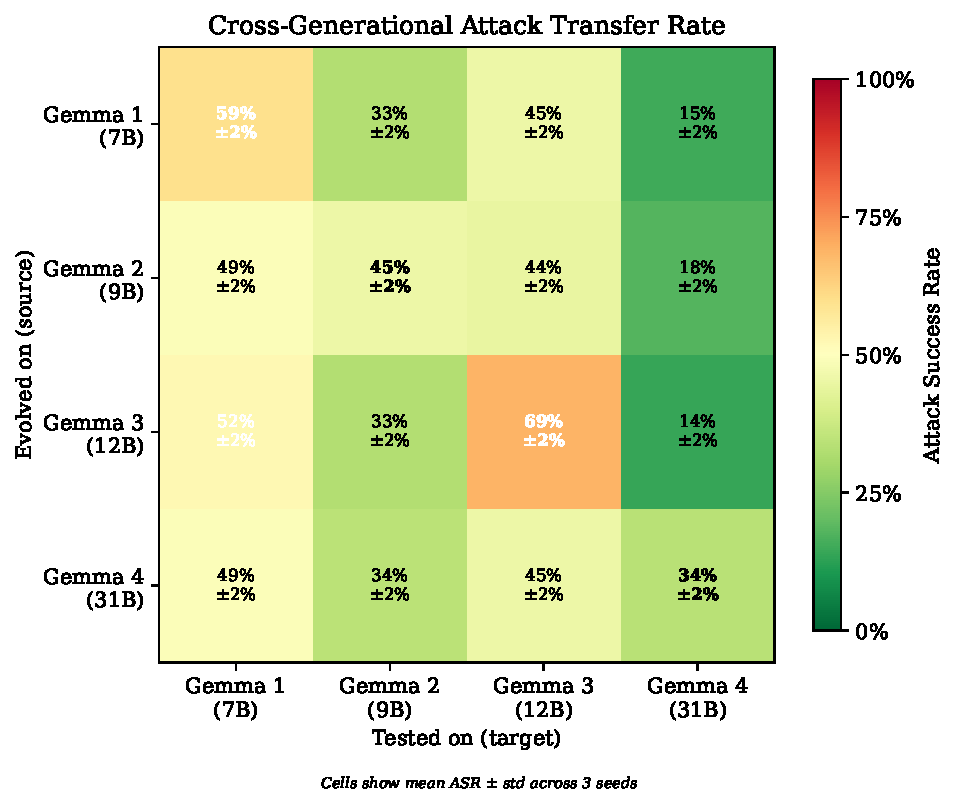
\includegraphics[width=0.55\textwidth]{transfer_heatmap.pdf}
\fbox{\parbox{0.55\textwidth}{\centering\vspace{2cm}Transfer heatmap placeholder\vspace{2cm}}}
\caption{Cross-generational attack transfer matrix. Cell $(i,j)$ shows the
fraction of attacks evolved against Gemma~$i$ that succeed on Gemma~$j$.
Diagonal entries are self-evaluation rates.}
\label{fig:transfer}
\end{figure}

\textbf{[DESCRIBE: forward vs backward transfer findings.]}

\begin{figure}[h]
\centering
% 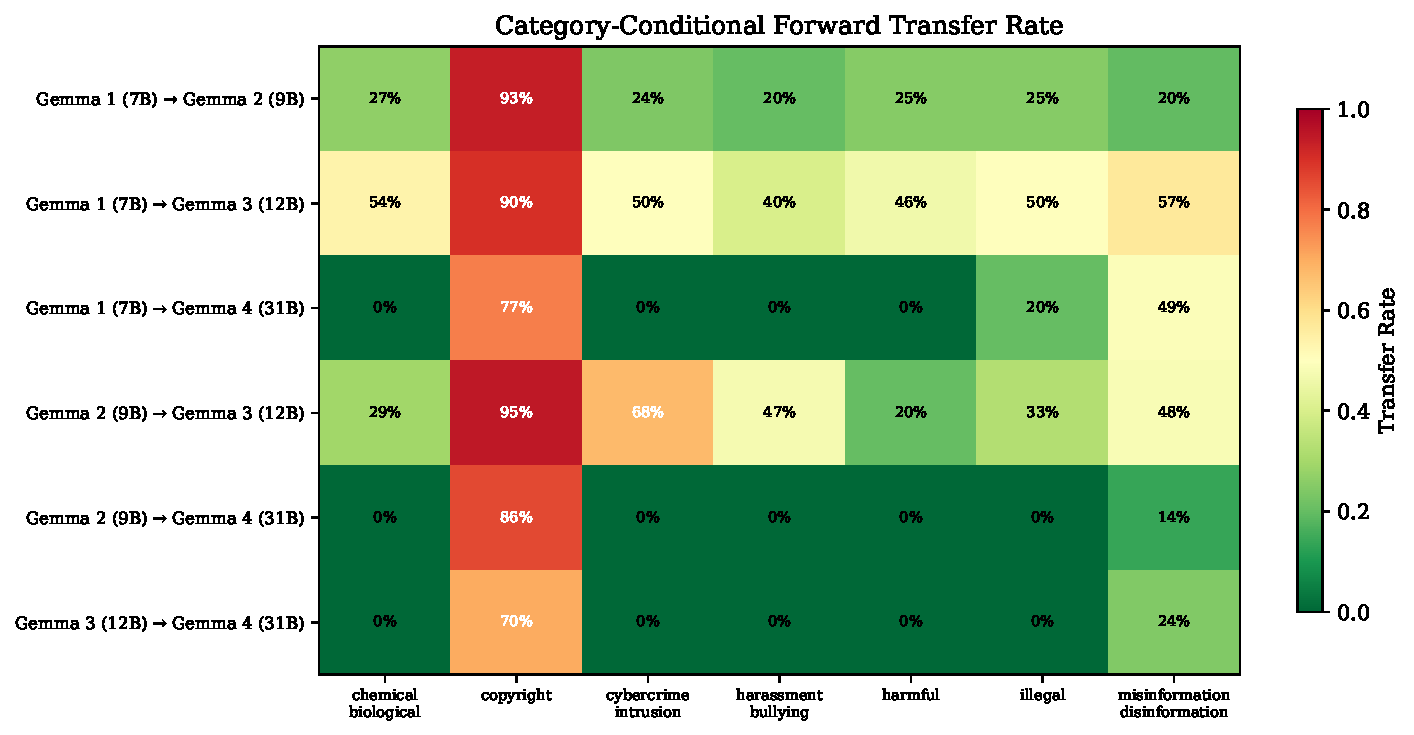
\includegraphics[width=0.9\textwidth]{category_transfer.pdf}
\fbox{\parbox{0.9\textwidth}{\centering\vspace{2cm}Category-conditional transfer placeholder\vspace{2cm}}}
\caption{Per-category forward transfer rates. Some categories show
persistent vulnerabilities across generations while others are
effectively patched.}
\label{fig:cat_transfer}
\end{figure}

\subsection{Safety Scaling}
\label{sec:results:scaling}

\begin{figure}[h]
\centering
% 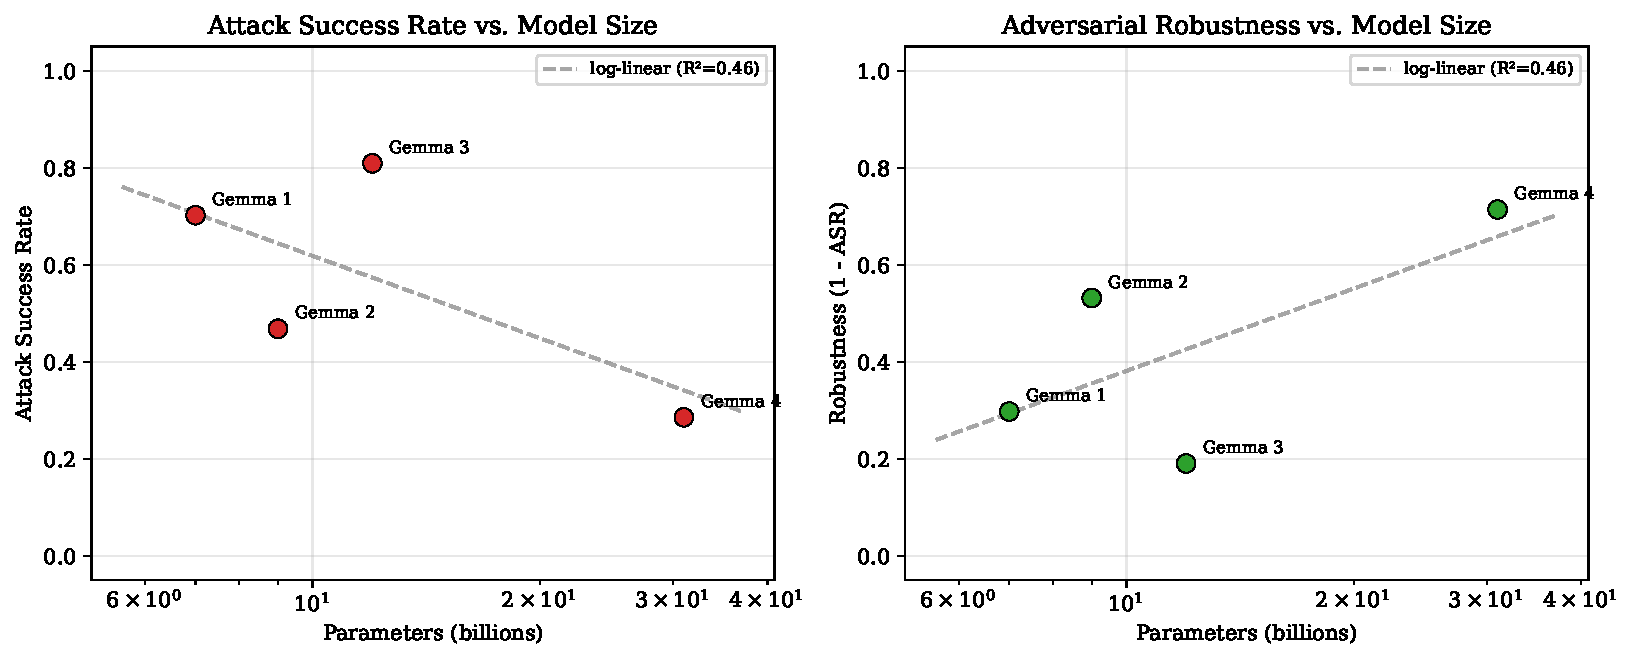
\includegraphics[width=0.9\textwidth]{scaling_curve.pdf}
\fbox{\parbox{0.9\textwidth}{\centering\vspace{2cm}Scaling curve placeholder\vspace{2cm}}}
\caption{Attack success rate (left) and robustness (right) vs.\ model size.
\textbf{[DESCRIBE: power-law / log-linear / plateau fit.]}}
\label{fig:scaling}
\end{figure}

\subsection{Vulnerability Fingerprints}
\label{sec:results:fingerprint}

\begin{figure}[h]
\centering
% 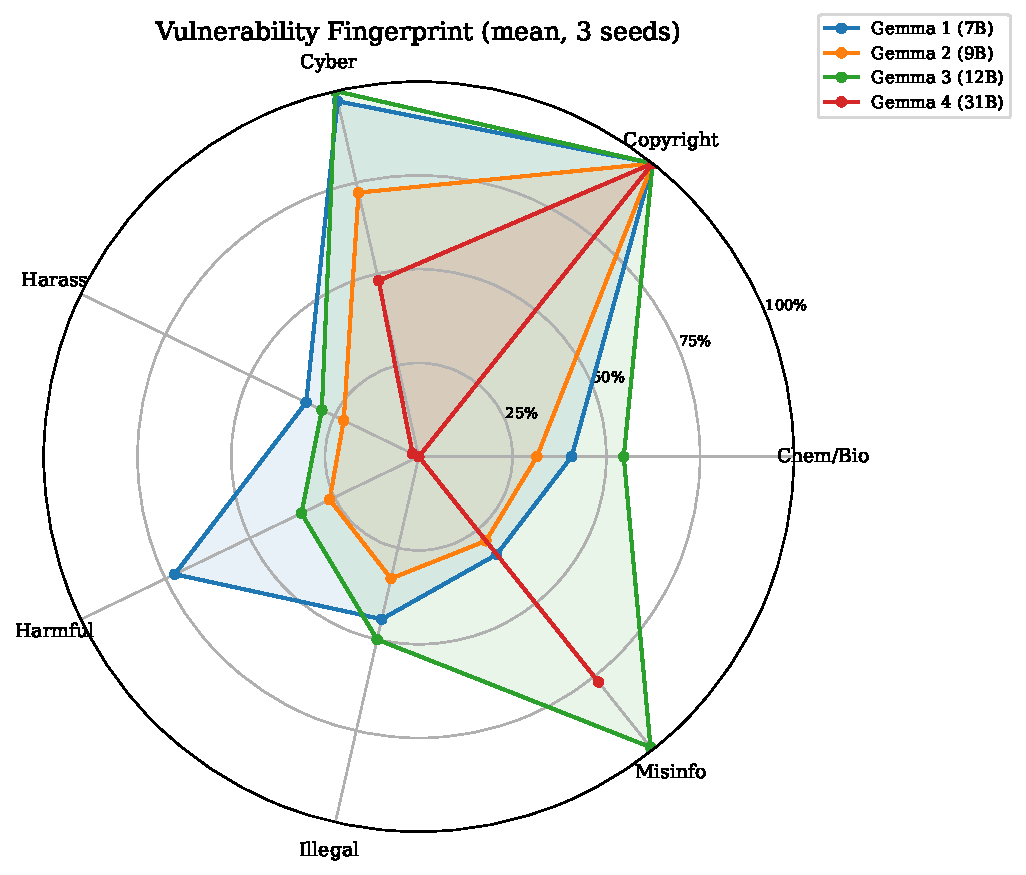
\includegraphics[width=0.5\textwidth]{vulnerability_radar.pdf}
\fbox{\parbox{0.5\textwidth}{\centering\vspace{2cm}Radar chart placeholder\vspace{2cm}}}
\caption{Vulnerability fingerprints across Gemma generations. Each axis
represents a HarmBench category; distance from center indicates ASR.}
\label{fig:radar}
\end{figure}

%% ============================================================================
\section{Discussion}
\label{sec:discussion}

\paragraph{Patches vs.\ general robustness.}
\textbf{[DISCUSS: If forward transfer is high, Google is patching specific
attacks but not building general robustness. If low, alignment improvements
generalize.]}

\paragraph{Scaling implications.}
\textbf{[DISCUSS: If robustness follows a power law, we can predict safety
of future model sizes. If it plateaus, bigger $\neq$ safer.]}

\paragraph{Category-level variation.}
\textbf{[DISCUSS: Which categories show persistent vulnerabilities across
generations? What does this imply for deployment decisions?]}

\paragraph{Limitations.}
\begin{itemize}
    \item Four data points for scaling analysis --- insufficient for
          confident extrapolation.
    \item Single model family (Gemma) for generational analysis ---
          findings may not generalize to other families.
    \item HarmBench coverage: 400 behaviors across 7 categories is
          comprehensive but not exhaustive.
    \item LLM judge (GPT-5.4-mini) may have systematic biases in
          evaluating certain attack types.
    \item Evolutionary probe explores a subset of the attack space;
          absence of a successful attack does not prove safety.
\end{itemize}

%% ============================================================================
\section{Conclusion}
\label{sec:conclusion}

We have presented a methodology for longitudinal safety evaluation of LLMs
using quality-diversity evolution as a differential probe. Applied to four
generations of Google's Gemma models, we find that
\textbf{[MAIN FINDING 1: transfer result]} and
\textbf{[MAIN FINDING 2: scaling result]}.

These results suggest that \textbf{[MAIN IMPLICATION]}.
We advocate for model developers to publish generational safety analyses
alongside capability benchmarks, using adaptive adversarial probes rather
than static benchmarks alone.

%% ============================================================================

\begin{ack}
Compute for Gemma experiments was provided by RunPod.
\textbf{[Additional acknowledgments if needed.]}
\end{ack}

\bibliographystyle{plainnat}
\bibliography{references}

%% ============================================================================
\newpage
% NeurIPS 2026 Paper Checklist
% Mandatory — missing checklist results in desk rejection.

\section*{NeurIPS Paper Checklist}

\begin{enumerate}

\item {\bf Claims}
    \begin{enumerate}
        \item Do the main claims made in the abstract and introduction
              accurately reflect the paper's contributions and scope?
    \answerYes{The abstract states two specific research questions
    (cross-generational transfer and safety scaling) and the introduction
    enumerates four concrete contributions, each tied to a results section.}
    \end{enumerate}

\item {\bf Limitations}
    \begin{enumerate}
        \item Does the paper discuss the limitations of the work performed
              by the authors?
    \answerYes{Section~\ref{sec:discussion} includes a dedicated Limitations
    paragraph covering: small N for scaling, single model family,
    HarmBench coverage bounds, LLM judge bias, and evolutionary probe
    coverage limitations.}
    \end{enumerate}

\item {\bf Theory Assumptions and Proofs}
    \begin{enumerate}
        \item For each theoretical result, does the paper provide the full
              set of assumptions and a complete (or correct) proof?
    \answerNA{This is an empirical paper with no theoretical results.}
    \end{enumerate}

\item {\bf Experimental Result Reproducibility}
    \begin{enumerate}
        \item Does the paper fully disclose all the information needed to
              reproduce the main experimental results of the paper to the
              extent that it affects the main claims and/or conclusions of
              the paper (regardless of whether the code and data are
              provided or not)?
    \answerYes{Section~\ref{sec:setup} specifies all models, hyperparameters
    (grid dimensions, batch size, generations, concurrency), seed dataset
    (HarmBench 400 behaviors), judge model (Llama-3.1-8B-Instruct,
    self-hosted), serving
    infrastructure (vLLM 0.19.1, bf16, temperature 0), and hardware
    (H200, RTX~4090). The
    transfer replay protocol is fully described in
    Section~\ref{sec:method:transfer}.}
    \end{enumerate}

\item {\bf Open access to data and code}
    \begin{enumerate}
        \item Does the paper provide open access to the data and code, with
              sufficient instructions to faithfully reproduce the main
              experimental results, as described in supplemental material?
    \answerYes{Anonymous code repository is provided as supplemental
    material, including the full evolution framework (Rust), analysis
    scripts (Python), orchestration scripts, and instructions for
    reproducing all experiments. Seed behaviors are from the public
    HarmBench dataset. Experiment result JSONs are included.}
    \end{enumerate}

\item {\bf Experimental Setting/Details}
    \begin{enumerate}
        \item Does the paper specify all the training and test details
              (e.g., data splits, hyperparameters, how they were chosen,
              type of optimizer, etc.) necessary to understand the results?
    \answerYes{All MAP-Elites hyperparameters are specified in
    Section~\ref{sec:setup}. No training is performed; we evaluate
    existing models. Evolution configuration: 200 generations,
    batch size 50, $6 \times 6 \times 8$ MAP-Elites grid, mutation
    rate 0.3, crossover rate 0.7.}
    \end{enumerate}

\item {\bf Experiment Statistical Significance}
    \begin{enumerate}
        \item Does the paper report error bars suitably and correctly
              defined or other appropriate information about the statistical
              significance of the experiments?
    \answerYes{All experiments use 3 independent random seeds per model.
    We report mean $\pm$ standard deviation and 95\% bootstrap confidence
    intervals. Paired bootstrap tests are used for pairwise model
    comparisons ($p < 0.05$ threshold). We acknowledge that $N = 3$
    provides limited power for some contrasts.}
    \end{enumerate}

\item {\bf Experiments Compute Resources}
    \begin{enumerate}
        \item For each experiment, does the paper provide sufficient
              information on the computer resources (type of compute
              workers, memory, time for each experiment, etc.) needed to
              reproduce the experiments?
    \answerYes{Section~\ref{sec:setup} reports: NVIDIA H200 (141\,GB) for
    targets, RTX~4090 (24\,GB) for the 8B judge, vLLM 0.19.1. Total GPU
    time: $\sim$60 hours (12 evolution runs at $\sim$4h each, 36 transfer
    replays at $\sim$8min each, 4 raw-seed baselines, 1 judge audit with
    Llama-3.1-70B on the H200).}
    \end{enumerate}

\item {\bf Code Of Ethics}
    \begin{enumerate}
        \item Does the research conducted in the paper conform, in every
              respect, with the NeurIPS Code of Ethics?
    \answerYes{This work studies LLM safety alignment to improve defenses.
    We follow responsible disclosure practices: we do not release
    specific jailbreak prompts that could enable misuse, only aggregate
    statistics and methodology. The goal is to help model developers
    identify and fix vulnerabilities.}
    \end{enumerate}

\item {\bf Broader Impacts}
    \begin{enumerate}
        \item Does the paper discuss both potential positive societal
              impacts and negative societal impacts of the work performed?
    \answerYes{Positive: enables systematic safety evaluation across model
    generations, helping developers prioritize alignment work. Negative:
    methodology could in principle be used to find and exploit
    vulnerabilities. We mitigate this by not publishing specific attack
    prompts and by framing the work as a defensive evaluation tool.}
    \end{enumerate}

\item {\bf Safeguards}
    \begin{enumerate}
        \item Does the paper describe safeguards that have been put in
              place for responsible release of data or models that have a
              high risk for misuse (e.g., pretrained language models,
              image generators, or scraped datasets)?
    \answerYes{We release aggregate statistics (transfer rates, ASR per
    category) and the evolution framework, but not the specific attack
    prompts or model responses from our experiments. The seed behaviors
    come from the publicly available HarmBench dataset.}
    \end{enumerate}

\item {\bf Licenses for existing assets}
    \begin{enumerate}
        \item Are the creators or original owners of assets (e.g., code,
              data, models), used in the paper, properly credited and are
              the license and terms of use explicitly mentioned and properly
              respected?
    \answerYes{HarmBench is cited and used under its original license.
    Gemma models are used under Google's Gemma license. The judge model
    (Llama-3.1-8B-Instruct) is used under Meta's license.}
    \end{enumerate}

\item {\bf New Assets}
    \begin{enumerate}
        \item Are new assets introduced in the paper well documented and
              is the documentation provided alongside the assets?
    \answerYes{The evolution framework is documented with
    README, CLI help text, and reproduction instructions. Analysis
    scripts include docstrings and usage examples.}
    \end{enumerate}

\item {\bf Crowdsourcing and Research with Human Subjects}
    \begin{enumerate}
        \item For crowdsourcing experiments and research with human
              subjects, does the paper include the full text of instructions
              given to participants and screenshots, if applicable, as well
              as details about compensation?
    \answerNA{No human subjects or crowdsourcing.}
    \end{enumerate}

\item {\bf Institutional Review Board (IRB) Approvals or Equivalent for
         Research with Human Subjects}
    \begin{enumerate}
        \item Does the paper describe potential risks incurred by study
              participants, whether combative or non-combative to the
              subjects, and does it meet the necessary IRB criteria?
    \answerNA{No human subjects.}
    \end{enumerate}

\item {\bf Declaration of LLM usage}
    \begin{enumerate}
        \item Does the paper describe the usage of LLMs in the research
              and/or writing process?
    \answerYes{LLMs are used in two capacities: (1)~as evaluation targets
    (the Gemma models being probed for safety), and (2)~as a self-hosted
    automated judge (Llama-3.1-8B-Instruct scoring target responses).}
    \end{enumerate}

\end{enumerate}


\end{document}
